\documentclass{article}
\usepackage[T1]{fontenc}
\usepackage{lmodern}
\usepackage{graphicx}
\usepackage{amsmath,amssymb}
\usepackage[a4paper,margin=2cm]{geometry}
\usepackage[absolute,overlay]{textpos}
\setlength{\TPHorizModule}{1mm}
\setlength{\TPVertModule}{1mm}
\usepackage[indonesian]{babel}
\usepackage{hyperref}
\setlength{\emergencystretch}{2em}
% unit: Halaman 15

\begin{document}

% === Halaman 15 (llm) ===

\vspace{205.23mm}

\begin{itemize}
    \item Selama kalkulasi plainteks menjadi cipherteks, status data sekarang disimpan di dalam matriks dua dimensi, \texttt{state}.
    \item \texttt{state} bertipe \textit{byte} dan berukuran $Nrows \times Ncols$
    \item Untuk blok data 128-bit, ukuran \texttt{state} adalah $4 \times 4$, seperti gambar di samping.
\end{itemize}

% deskripsi: Diagram yang menunjukkan transformasi plainteks 128-bit menjadi matriks state berukuran 4x4.
% bbox normalisasi: [0.6450, 0.1940, 0.8980, 0.8850]
\begin{textblock*}{53.13mm}(135.45mm,57.62mm)
\noindent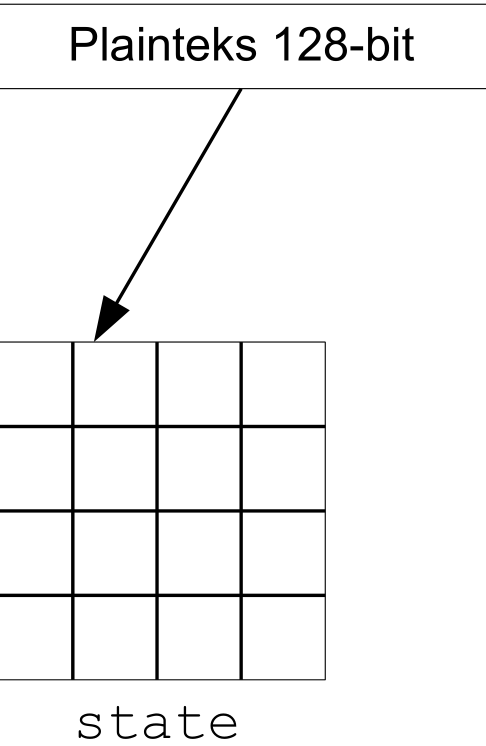
\includegraphics[width=53.13mm,height=205.23mm]{../../images/llm/page_015_img_01.png}%
\end{textblock*}

\end{document}
